\red{
\begin{itemize}
	\item \textbf{Make this section everything \underline{after first flight}}
	\item Development of basic flight systems after construction of airframe
	\item Discuss Prototype \#1
	\item Testing of basic flight with Prototype
	\item testing:validation(how we knew we could fly), iterative design (designs changed through testing (like the back gears)), and problems (like the motor, power module and radio, their effect, and how they were resolved), link to diary (as there were significant set backs)... mention optimal 3D print orientations were investigated to strengthen against most possible failure modes.
\end{itemize}}

\subsection{Prototype 1 ``Scorpion''}
Initially, development on the Skywalker X8 was postponed, and a replaceable foam model developed, so that problems (and damage) did not result in significant cost and delays to the project. Many of the initial flight tests were conducted on our first prototype, "The Scorpion" (see Figure \ref{fig:balance_table}).

\subsection{Prototype 2 ``Dragonfly''}
Once the configuration of parts had been tested together and the scorpion had undergone some basic flight tests, the parts were moved onto the Skywalker X8. Some additional modifications were required such as rings for the front pole in between the layers of foam, and custom pole mounts. Table \ref{tab:tests} in Appendix \ref{sec:diary} shows major flight tests conducted on 'The Dragonfly'. A maximum hover time of 15 minutes has so far been achieved with battery life still left over.  

\subsection{Testing Mechanisms}
\subsubsection*{Thrust:} In order to achieve the greatest lift for take-off, a number of tests were conducted on the rig (shown in Figure \ref{fig:rig}) to measure the relative force of various propeller sizes and materials. Table \ref{tab:props} summarizes the results, which indicate that the 12$\times$6 APC (Plastic) blades produce the greatest force, and are best suited for take-off. Each propeller is able to pull over 2.02kg. Collectively, the 6kg of thrust from the 3 motors (even from non-calibrated ESCs) is more than enough for the craft, which is under 4kg, to take off. The recommended Pixhawk hover throttle of under 80\% is also achieved  


\red{move this table to appendix}
\begin{table}[htbp]
	\centering
	\begin{tabular}{|c|c|c|c|}
		\hline Material & Dimensions & Measurements & Average Force (kg) \\ 
		\hline Carbon fibre & 12$\times$6 & [1.685, 1.695, 1.692, 1.690. 1.700] & 1.692 \\ 
		\hline Carbon fibre & 11$\times$5.5 & [0.635, 0.635, 0.635, 0.635, 0.635] & 0.635 \\ 
		\hline APC (Plastic) & 12$\times$6 & [1.965, 2.030, 2.030, 2.020, 2.045] & 2.02 \\ 
		\hline APC (Plastic) & 11$\times$5.5 & [1.645, 1.630, 1.625, 1.620 1.620] & 1.628 \\ 
		\hline 
	\end{tabular} 
	\caption{Measurements of propeller performance}
	\label{tab:props}
\end{table}

\begin{figure}[!ht]
	\centering
	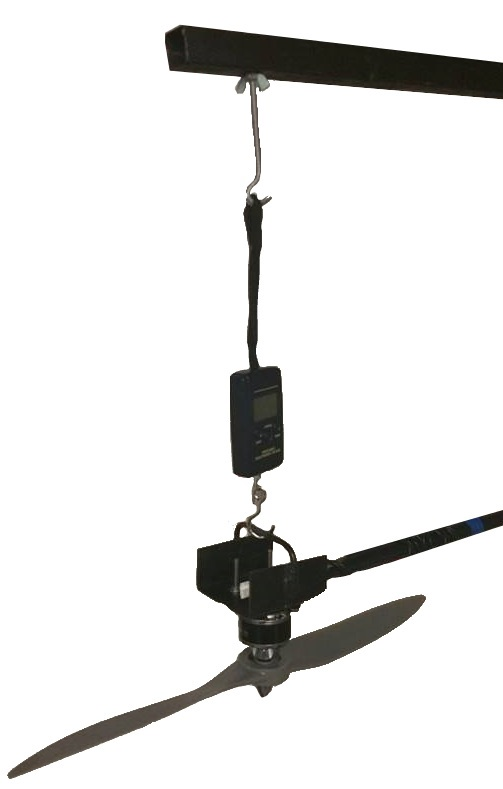
\includegraphics[width=200pt]{\IMAGEPATH /Prototype/rig}
	\caption{Thrust testing rig}
	\label{fig:rig}
\end{figure}



\subsubsection*{Balance Table:} The craft was placed on a table that can rotate in all 3 axis to ensure it was capable of stabilising itself. This also acted as a good way to measure the strengths and weaknesses of the parts when they needed to be tested. 

\begin{figure}[!ht]
	\centering
	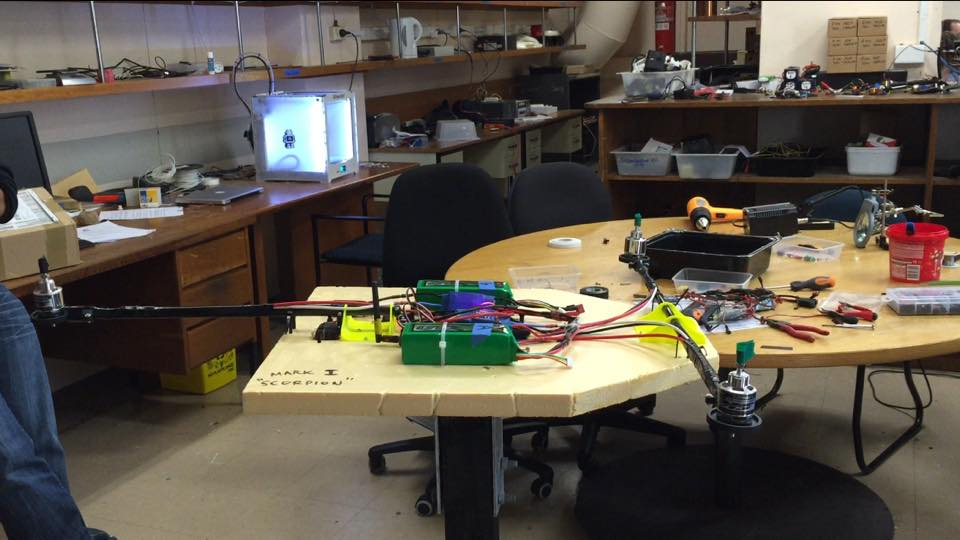
\includegraphics[width=200pt]{\IMAGEPATH /Prototype/balance_table}
	\caption{The Scorpion on the balance table}
	\label{fig:balance_table}
\end{figure}


\subsection{Iterative Design}
Through testing mechanisms and flight tests, a number of problems with the aircraft have been tweaked and resolved

\subsubsection*{Vibrations:} Numerous vibration related problems and set-backs were encountered during testing and evaluation of the prototypes. To combat this, an assortment of nyloc-nuts and spring-washers were utilized in order to fasten components together in a vibration resistant manner. The addition of four rubber ``feet'' to the base of each motor succeeded in damping any vibratory response down the pole shaft. Overall this was extremely effective in increasing stability, as vibrations appeared to mitigated in follow-up tests.

\subsubsection*{Motor Mounts:} As previously mentioned there had been many iterations of motor mount design. This is due to the numerous problems that were resolved to do with strength, vibration and fastening of the mounts. The final design addresses all issues. One test that was conducted extensively was the affect if the orientation of the motor mount prints. It was found that printing the layers on the same plane as both the bar and the direction of force gave the most strength. This is because the layer plane is in the same direction as the moment and they are not being pulled apart in any way. See table \ref{tab:back_mount}.

\subsubsection*{Gears:} Initially 1:2 gear ratios were chosen for both front and back gear systems. Through testing however, it became evident that the servos could power a 1:1 system which allowed for larger teeth and hence overall strength see table \ref{tab:minor}.

\subsubsection*{Wires and Soldering:}  A major problem discovered was high temperatures causing solder to melt and connections to be lost. This resulted in system wide power loss. This was resolved by changed to non-lead based solder, increased melting temperatures by 40 degrees, ventilating the craft, and using higher spec wiring. 

\subsubsection*{Radio Failure:} Problems were encountered with the initial remote control  transmitter leading to strange behaviour in flight. Range tests were conducted, and they are believed to be faulty. The back up transmitter (HK-T6A V2) was chosen and resolved these problems.

\subsubsection*{Motor Failure:} Mid-flight motor failure was encountered causing complete aircraft failure with many parts requiring repair. It is unknown whether this was caused due to manufacturing error in the motors, or debris flying into it. Either way future flights have been conducted with little debris and grass that cannot reach the propellers. 

\subsubsection*{Power Module Failure:}  The initial 3DR Power Module received was faulty and a cheaper third party one was used for a few flights. Extremely unpredictable behaviour of the craft followed, and led to another major crash. After many sensor, current and voltage tests it was determined to be the power module. A new 3DR Module was purchased, and no issues have ensued since.\\  

See Table \ref{tab:tests} in Appendix \ref{sec:diary} for test flight dates.
